% little trick to replace lib.tex by this
\renewcommand{\doctitle}[1]{
	\chapter{#1}
}
\renewcommand{\biblio}[1]{}
\doctitle{Le filtre}
Le filtre utilise la propriété des diodes de ne laisser passer 
le courant qu'à partie d'une certaine tension. Grâce à cela,
l'on peut faire un diviseur de tension qui varie en fonction 
de la tension lui étant appliquée. 

\begin{figure}[ht]
	\centering
	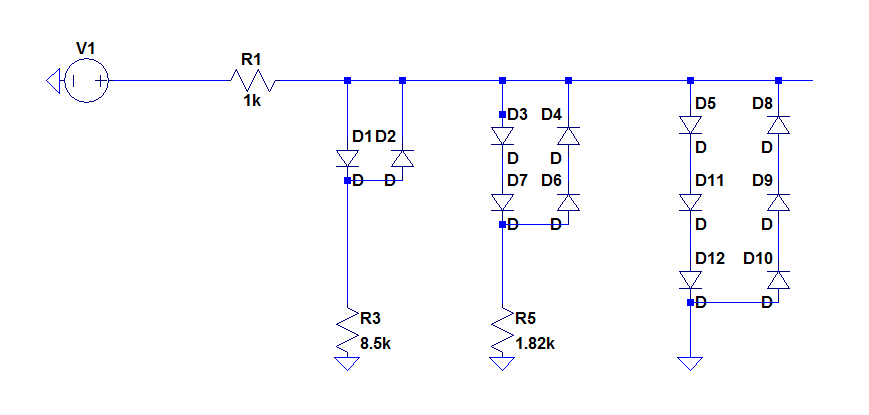
\includegraphics[scale=0.4]{img-filter/filter-circuit.jpg}
	\caption{Circuit du filtre.}
	\label{fig:filter-spice-graph}
\end{figure}

\begin{figure}[ht]
	\centering
	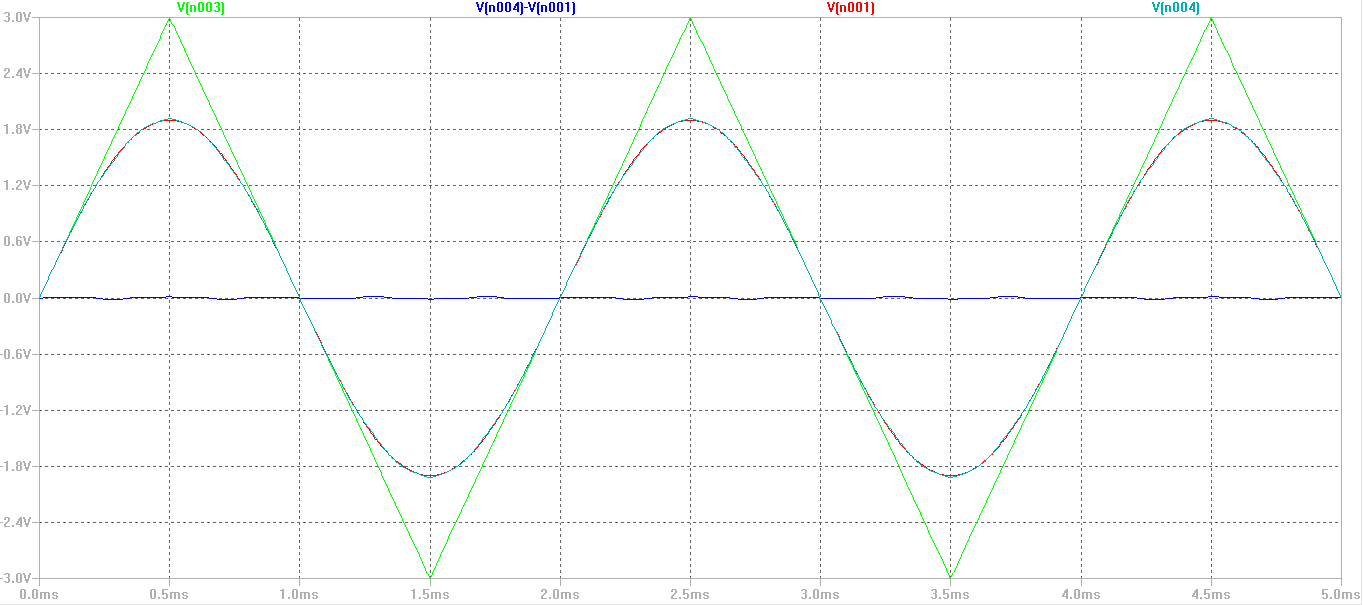
\includegraphics[scale=0.3]{img-filter/filter-spice-graph.jpg}
	\caption{Simulation du filtre. En vert l'entrée triangulaire. La
	sortie est superposée (et confondue) à un vrai sinus.}
	\label{fig:filter-spice-graph}
\end{figure}

\end{document}